\documentclass[12pt]{article}
\usepackage{lastpage, fancyhdr,color,amsmath,amssymb,amsfonts,amscd, graphicx,latexsym}
\usepackage{eurosym}
\usepackage[all]{xy}
\pagestyle{empty}
%\usepackage[turkish]{babel}
\usepackage[utf8]{inputenc}
\usepackage[T1]{fontenc}
\setlength\voffset{-1in}
\setlength\hoffset{-1in}
\setlength\topmargin{3cm}
\setlength\oddsidemargin{2.5cm}
\setlength\textheight{8in}
\setlength\textwidth{6.51in}
\setlength\footskip{1in}
\setlength\headheight{12pt}
\setlength\headsep{0.06in}
\usepackage{tikz}
%plus4mm minus3mm}
\usepackage{caption, subcaption, amsfonts}
\usepackage{setspace}
\usepackage{epstopdf}
\usepackage{relsize}
\usepackage{pgf, float}
\usepackage{url}
\newcommand{\gal}{Gal({\mathbb Q})}
\newcommand{\N}{\mathbb N}
\newcommand{\F}{\mathcal F}
\renewcommand{\H}{\mathcal H}
\newcommand{\Q}{\mathbb Q}
\newcommand{\Z}{\mathbb Z}
\newcommand{\R}{\mathbb R} 
\newcommand{\C}{\mathbb C}
\newcommand{\p}{\mathbb P}
\newcommand{\B}{\mathbb B}
\def\modorb{\mbox{$\otimes\hspace{-1.5mm}-\!\!\!-\!\!\!-\hspace{-1.5mm}\circledast$}}
\hyphenation{or-bi-fold}
%\input{defs.tex}

%\usepackage[usenames,dvipsnames]{color}
%\usepackage{epsfig}


% ’

\definecolor{light-gray}{gray}{0.55}
\newcommand\Note[1]{\textcolor{red}{{#1}}}
\begin{document}
\pagestyle{fancy}
   \lhead{}\rhead{}
   \lfoot{\textcolor{light-gray}{\small Proje Sonuç Raporu}}
        \rfoot{\textcolor{light-gray}{\small Sayfa {\thepage}}}
        \cfoot{}
  \renewcommand{\headrulewidth}{0pt}
%  \renewcommand{\footrulewidth}{0.4pt}
%\def\HG{{\bf HG-GalAct }}

\label{coverpage}

\renewcommand{\figurename}{Şekil}
\renewcommand{\tablename}{Tablo}
\renewcommand{\contentsname}{İçindekiler}
\renewcommand{\refname}{Referanslar}

\newpage
\phantom{22}
\vspace{-3cm}

% % % {\selectlanguage{turkish}\bfseries\color{red} \small Başvuru Formunun ``Bütçe ve Gerekçesi (13. Madde)'' dışındaki bölümleri toplamda Arial, 9 yazı tipinde 20 sayfayı geçmemelidir!}
% % % 
% % % \begin{center}
% % % 	\selectlanguage{turkish}\bfseries \footnotesize Kariyer proje önerisi değerlendirme formuna \\ \url{http://www.tubitak.gov.tr/tubitak_content_files/ARDEB/destek_prog/danisman_panelist/3501_DA_Panelist_Proje_Onerisi_Degerlendirme_Formu.doc} \\
% % % 	adresinden ulaşabilirsiniz.
% % % \end{center}


\begin{center}

\includegraphics[keepaspectratio]{tubitak.png}

\bigskip
\bigskip


\bigskip
{\fontsize{15}{10}\selectfont 
\bigskip


\bigskip
\medskip
{ \textbf{\Huge Birden Fazla Veri Kaynağı Kullanabilen Yeni Genom Birleştirme Algoritmalarının Tasarımı Ve Uygulanması \\}}}


\bigskip
\medskip
{ \textbf{ PROJE SONUÇ RAPORU}}
\bigskip





\end{center}


\bigskip

\bigskip


\thispagestyle{empty}


\begin{center}
\medskip
{\LARGE \textbf{Program Kodu:} 1001}

\bigskip
{\LARGE \textbf{Proje No:} 112E135}

\bigskip
{\LARGE Proje Yürütücüsü:\\
\textbf{Can Alkan}}

\end{center}



\bigskip


\bigskip
\noindent
{\Large
\noindent
\underline{\bf Bursiyerler:}

\noindent
Shatlyk Ashyralyyev

\noindent
Fatma Balcı (Kahveci)

\noindent
Elif Dal


}



\bigskip





\begin{center}
{\Large EYLÜL 2015

\vspace{1mm}
ANKARA}
\end{center}


\linespread{1.5}

\newpage\setlength{\parskip}{3mm} 
\onehalfspacing
\bigskip
\setcounter{page}{1}
\begin{center}
{\LARGE \bf ÖNSÖZ}
\end{center}
\addcontentsline{toc}{section}{ÖNSÖZ}


Proje süresince proje ekibinin şu yayınları hazırlanmıştır: 

\begin{itemize}
\item Early post-zygotic mutations contribute to de novo variation in a healthy monozygotic twin pair. G.M. Dal, B. Ergüner, M. S. Sağıroğlu, B. Yüksel, O. E. Onat, {\bf C. Alkan}, T. Özçelik. Joural of Medical Genetics, 51:455-459, 2014.
\item Whole genome sequencing of Turkish genomes reveals functional private alleles and impact of genetic interactions with Europe, Asia and Africa. {\bf C. Alkan}, P.  Kavak, M. Somel, O. Gokcumen, 
  S. Uğurlu, C. Saygı, {\bf E. Dal}, K. Buğra-Bilge,  T. Güngör, S. C. Sahinalp, N. Özören, C. Bekpen. BMC Genomics, 15(1):963, 2014.
\end{itemize}

Proje süresince proje ekibinin şu bildiriler sunulmuştur:
 
\begin{itemize}
\item A hypergraph model for hybrid genome assembly. {\bf S. Ashyralyyev}, C. Firtina, C. Aykanat, {\bf C. Alkan}. Bertinoro Computational Biology Meeting, 14-18 May 2015, Bertinoro, Italy.

\end{itemize}

Proje kapsamında desteklenen aşağıdaki bursiyerler,  lisansüstü eğitimlerini 
proje yürütücüsünün danışmanlığında
yapmıştır.
 
\begin{itemize}
\item Fatma Kahveci (Balcı), Bilkent Üniversitesi Bilgisayar Mühendisliği, Yüksek Lisans, Ağustos 2014.
\item Elif Dal, Fatma Kahveci (Balcı), Bilkent Üniversitesi Bilgisayar Mühendisliği, Yüksek Lisans, Aralık 2014.
\end{itemize}


\bigskip
\hfill Can Alkan

\hfill Ankara, Eylül 2015
\newpage

\setlength{\parskip}{1mm} 

\tableofcontents


 



\newpage \setlength{\parskip}{3mm}
\phantom{ss}
\vspace{-2.5cm}

\begin{center}
{\bf \Large ÖZET} 
\end{center}
\addcontentsline{toc}{section}{ÖZET}
\noindent

Yeni nesil dizileme (YND) teknolojilerinin uygulanmasi genomiks alanını kökten değiştirmektedir. Farklı türlerin genomlarini incelemede ve gerek normal gerekse hastalığa yol açan insanlardaki genetik farklılıkların incelenmesinde önceden beklenmeyen derecede çözünürlük sağlamaktadır. Her ne kadar YND verilerinin analizi için çok önemli gelişmeler olmuşsa da, halen YND yöntemlerinin tüm gücünden faydalanılmasının önünde engeller vardır.

Önceden hayal dahil edilemeyecek hızda verileri günümüzde üretebiliyor olmamıza rağmen, bu verilerin analizleri çok daha yavaş hızda olmaktadır. Çünkü 1) emsalsiz miktarlardaki veriler bilişimsel altyapılarda hem verilerin saklanması hem de işlenmesi açısından sorunlar doğurmaktadır; 2) YND platformları tarafından üretilen dizi parçaları genelde yüksek oranda hata içermektedir ve bu parçalar çok kısadır; 3) hem halihazırda kullanılmakta olan algoritmalar hem de YND platformları genomun bazı farklı yapıdaki bölgelerinde düşük performanslı çalışmaktadırlar. İşte bu nedenlerden ötürü dizileme verilerinde var olan bilgiler tamamen kullanılamamaktadır. Bu çok miktardaki verilerin daha iyi işlenmesi ve YND yöntemlerinin gerçek gücünün ortaya çıkarılması için bilgisayar bilimleri ve genomiks arasında bir işbirliğinin kurulması gerekmektedir.

Genom dizileme maliyetinin büyük ölçüde düşmesi sayesinde farklı organizmalar arasındaki genomik çeşitliliğin, organizmal biyolojinin ve genom evriminin daha iyi anlaşılması için binlerce farklı türün genomlarının dizilenmesine yönelik büyük bir ilgi vardır. Son bir kaç yılda bir çok genom, örneğin pirinç, üzüm, buğday, patates, mısır ve salatalık gibi bitkiler; panda, hindi, goril, orangutan, bonobo, keseli sıçan (opossum) ve fil gibi hayvanların genomlari dizilenmistir. Yakın zamanda Genome 10K gibi çok iddialı projeler başlamış ve 10.000 omurgalı hayvanın tüm genom dizilenmesinin yapılması amaçlanmıştır. Ancak YDS platformlarıyla üretilen verilerin yukarıda bahsedilen sınırları farklı türlerin referans genomlarının ortaya çıkarılmasını amaçlayan yeni dizileme çalışmalarını da (de novo sequencing) olumsuz etkilemektedir. Bunun başlıca nedenleri çoğu türün genomlarında aynı ya da benzer DNA dizilerinin genomun farklı yerlerinde tekrarlanması, YND verilerindeki dizi parçacıklarının (sequence read) kısa olması ve yüksek oranda hataların bulunmasıdır. Bu nedenle tüm genom dizilerinin çıkarılması sırasındaki genom birleştirmenin (genome assembly) doğruluğunun arttırılması için halen çözülmesi gereken problemler bulunmaktadır. Dizilenmiş genomların doğruluğu yetersiz derecede olursa, bu genomların incelenmesinden çıkarılacak biyolojik sonuçlar da hatalı olacaktır.

Bu projede birden fazla veri türünü birlikte kullanabilecek algoritmaların tasarlanmasını ve uygulanmasını hedefledik. Farklı şekillerde üretilmiş genom dizileme verilerinin gösterdiği farklı özellikleri aynı anda kullanarak ortaya çıkarılacak referans genomlarının kalitesinin arttırılması için çeşitli yöntemler üzerinde çalıştık. Böylece bu proje dahilinde üretmeye başladığımız gelişmiş algoritmalar yeni dizilenmiş genomları daha iyi birleştirmemizi sağlayacak ve genom biyolojilerini daha iyi anlamamıza yardımcı olacaktır. 

Bu proje dahilinde üç ana amaç üzerinde çalıştık. Birincisi Illumina platformunda ortaya çıkan GC oranlarının yüksek ve düşük olduğu bölgelerdeki dizileme derinliğindeki sapmaların düzeltilmesi ve özellikle ekzom dizilemedeki hataların giderilmesi, böylece ekzom birleştirmelerinin iyileştirilmesidir (Fatma Balcı, Yüksek Lisans Tezi). İkincisi, önceden geliştirilmiş olan iskeleleme algoritmalarının birden fazla veri tipi ve havuzlanmış klon dizileme verileri kullanıldığında genom birleştirmelerine faydalı etkisinin incelenmesiydi (Elif Dal, Yüksek Lisans Tezi). Son olarak Illumina verileri kullanılarak PacBo verilerindeki hataların düzeltilmesi (Can Fırtına, Yüksek Lisans Tezi -- sürüyor) ve düzeltilmiş PacBio verileri ile Illumina verilerinin eşzamanlı olarak bir hiperçizge üzerinde ifadesi ile genom birleştirmesi yapılmasıdır (Shatlyk Ashyralyyev. doktora tezi -- sürüyor).

{\bf Anahtar kelimeler:} genomiks, yeni nesil dizileme, genom birleştirme, algoritmalar, çizge kuramı

\newpage
\phantom{ss}
\vspace{-2.5cm}


\begin{center}
{\bf \Large ABSTRACT}
\end{center}
\addcontentsline{toc}{section}{ABSTRACT}
\noindent
The application of high throughput sequencing (HTS) technologies are revolutionizing the field of genomics, providing unprecedented resolution to study genomes of different species, and normal and disease causing human genetic variation. Although significant advances have been made to analyze HTS data, there are still several hurdles in fully utilizing the power of HTS. 

Although we can now generate data at a rate previously unimaginable, the analysis of the data is proceeding at a slower pace because: 1) unprecedented amounts of data introduce challenges in computational infrastructure in terms of both storage and processing power; 2) reads are often associated with high sequence errors and shorter read length; and 3) currently available algorithms to analyze HTS data and the HTS data themselves show different biases against different regions of the genome. Due to these problems, the information available in the sequencing datasets is not completely mined. There is a need to forge an alliance between computer science and genomics to devise better methods to use the massive amount of sequence data to unleash the full power of HTS methodologies.

Thanks to the substantially reduced cost of genome sequencing, there is now great interest in sequencing the genomes of thousands of species to better understand the genomic diversity across different organisms, organismal biology and genome evolution. In the last few years many genomes are sequenced: plants such as rice, grape, wheat, potato, corn, cucumber; and animals such as the giant panda, turkey, gorilla, orangutan, bonobo, opossum, elephant, etc. Recently more ambitious projects like the Genome 10K Consortium are started to sequence the genomes of 10.000 vertebrate species. However, the aforementioned limitations of the HTS technologies also affected de novo sequencing studies that aim to construct the reference genomes of various species. This is mainly due to the repetitive structure of the genomes of most species, the short sequence reads generated by current platforms, and the increased error rate. Thus there are still problems to solve to increase the accuracy of the assembled genomes; otherwise any biological conclusions derived from non-accurate genome assemblies would be incorrect.

Reasoning from the previous observations and empirical evidence that all current HTS platforms show different strengths and biases, we proposed to devise novel genome assembly algorithms that use data from multiple sources, including, when available, data derived from laboratory experiments to better assemble the genomes of new species. We aimed to test our algorithms with 1) a set of bacterial artificial chromosomes (BACs) generated from a hydatidiform mole resource that were sequenced using both the Illumina and Pacific Biosciences platforms, and test the assembly accuracy by comparing with high quality assemblies of the same resource using capillary sequence data; 2) whole genome shotgun sequence libraries generated from a haploid genome (hydatidiform mole) and sequenced using 454/Roche and Illumina platforms, several BAC end sequences from the same library sequenced using capillary sequencing, and physical fingerprinting data. The basepair calling accuracy of the Illumina platform coupled with longer matepairs from the 454/Roche, long sequences from Pacific Biosciences, long ``jumps'' from BAC end sequencing are being used in harmony to improve the genome assembly. In long the term, during a future project, we will also incorporate methodologies that utilize data from upcoming nanotechnology-based sequencing platforms such as the Oxford Nanopore Technologies. Enhanced algorithms that can better assemble genomes will improve our understanding of the biology of genomes.

In this project, we worked on three main aims. First, we developed methods to correct for GC bias associated with the Illumina platform together with biases due to exome capture efficiency to help fix errors in exome assemblies (Fatma Balcı, M.Sc. thesis). Next, we investigated the efficacy  of current scaffolding algorithms when data from multiple sequencing platforms are used together with pooled clone sequencing data (Elif Dal, M.Sc. thesis). Finally, we are continuing to work on Illumina-based error correction for Pacific Biosciences reads (Can Fırtına, M.Sc. thesis -- in progress), and a novel genome assembly algorithm by simultaneously representing Illumina and Pacific Biosciences reads on a hypergraph (Shatlyk Ashyralyyev, Ph.D. thesis -- in progress).

{\bf Keywords:} Genomics, high throughput sequencing, genome assembly, algorithms, graph theory


\newpage
\begin{center}
{\bf \Large 1. GİRİŞ}
\end{center}
\addcontentsline{toc}{section}{1. GİRİŞ}

\bigskip
\noindent
{\bf \large 1.1 }
\addcontentsline{toc}{subsection}{1.1 }

\noindent

\begin{center}
{\bf \Large 2. LİTERATÜR ÖZETİ}
\end{center}
\addcontentsline{toc}{section}{2. LİTERATÜR ÖZETİ}

Birkaç yıl önce piyasaya çıkan yeni nesil dizileme (YND) platformları sayesinde genom dizileme fiyatı milyonlarca kez ucuzlamış, ve genom bilimleri alanında yeni bir çığır açılmıştır~\cite{Mardis2008}. 15 yıl süren insan genom projesi 3-10 milyar Amerikan dolarına mal olmuşken, hem dizileme teknolojileri hem de genel dizileme yöntemlerinin (hiyerarşik dizileme yerine tüm genom dizileme) değişmesi ile bu miktar 2007 yılında 10 milyon dolar seviyesine, 2008'de 2 milyon dolara ve bugün 10 bin dolar altına düşmüştür (Şekil~\ref{fig:cost})

\begin{figure}[htb]
\begin{center}
  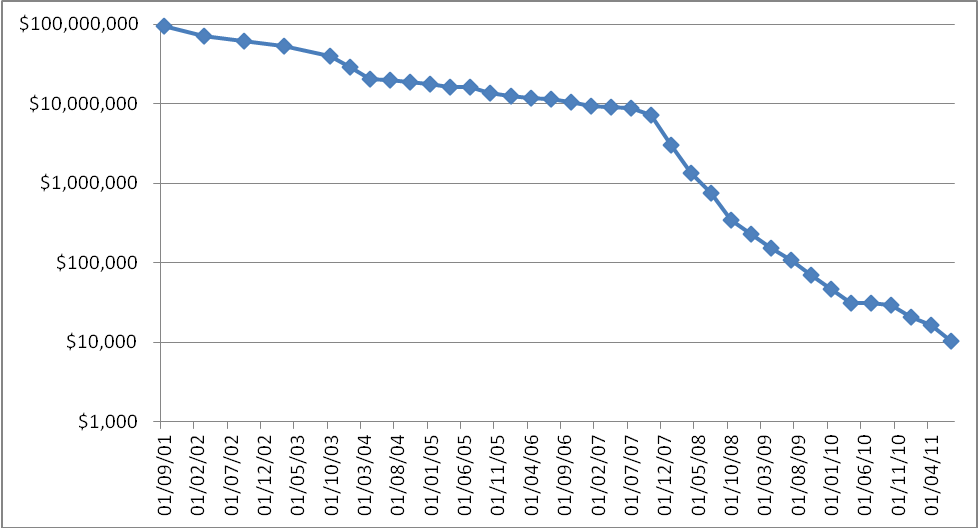
\includegraphics[scale=0.75]{cost.png}
\end{center}
\caption{Yıllara göre genom dizileme maliyetindeki değişimler. http://www.genome.gov/SequencingCosts/ adresinden alınmıştır.}
\label{fig:cost}
\end{figure}


Şu anda kullanılmakta olan birçok farklı ikinci ve üçüncü nesil YND platformu vardır. Bunların başlıcaları olarak 454 Life Sciences şirketinin ürettiği GS FLX sistemi, Illumina şirketinin ürettiği HiSeq2000/HiSeq2500/HiSeq3000/HiSeq4000, Ion Torrent'in PGM ve Proton, Pacific Biosciences'in SMRT teknolojisi ve PacBio RS platformu, Applied Biosystems'in SOLiD cihazı olarak listelenebilir. Çok daha yeni olarak nanoteknoloji temelli ``dördüncü nesil'' platformları (örn. Oxford Nanopore) piyasaya çıkmaya başlamıştır~\cite{Metzker2010,Loman2015}. Her ne kadar dizileme maliyeti çok düşmüşse de YND teknolojilerinin ürettiği verilerin bazı eksik yönleri vardır. Okunan ortalama dizi parçacığı uzunluğu çok kısa (örn. Illumina için 150 baz çifti), kullanılan DNA molekülleri çok küçük (örn. Illumina için 200-700 baz çifti), ve baz okuma hata oranı çok yüksek ve değişkendir (Illumina için \%0.1, Pacific Biosciences için \%15).


YND teknolojilerindeki baş döndürücü ilerleme, bu verilerin işlenmesine olan ihtiyaç nedeniyle bilgisayar bilimleri alanında da artan bir faaliyete neden olmuştur~\cite{Pop2008}. Elde edilen verilerin referans genomuyla karşılaştırılması ile değişik bireyler arasındaki genomik farklılıkların bulunması önemli bir araştırma alanıdır~\cite{Alkan2011,DePristo2011}. Bu nedenle 2.500 insan genomunun ayrıntılı incelenmesini amaçlayan 1000 Genom Projesi halen devam etmektedir~\cite{1000GP,1000GP2012}. Normal farklılıkların dışında genetik hastalıkların nedenlerinin bulunması için de YND platformları eşsiz bir güç sunmaktadır~\cite{Bamshad2011}. Ayrıca YND yöntemleri hücrelerdeki tüm RNA moleküllerinin tamamı anlamına gelen transkriptom dizilenmesi~\cite{Wang2009} ve genlerin aktivasyonlarini ölçmek~\cite{Park2009} için de kullanılabilir. 

Yukarıda belirtilenlerin dışında YND teknolojilerinin yoğunlukla uygulandığı bir alan da tüm genom dizileme birleştirmesi (de novo genome assembly) yoluyla farklı organizmaların referans genomlarının çıkarılmasıdır~\cite{Schatz2010}. Bugüne kadar geliştirilmiş olan genom birleştirme algoritmalarının hepsi çizge kuramı (graph theory) temellerine dayalı algoritmalardır. Başlıca iki tür genom birleştirme yöntemi vardır. Bunlardan ilki olan örtüşme çizgesi (overlap graph) yönteminde dizi parçaları çizgede uç olarak ifade edilir ve arasında başlangıç/sonuç ilişkisi olan dizi parçaları arasına kenar eklenir ve oluşan çizge üzerinde Hamilton turu (Hamiltonian path) aranır. Bu yöntemin örnekleri arasında eski nesil dizileme teknolojileri için kullanılan Celera Assembler~\cite{Myers2002}, Phusion~\cite{Mullikin2003} ve ARACHNE~\cite{Batzoglou2002} bulunur. İkinci ana yöntem genelde YND birleştirmelerinde kullanılan de Bruijn çizgesidir. Bu yöntemde YND dizi parçaları daha küçük ve aynı uzunlukta parçalara bölünür (k-mer), bu k-mer'ler çizgede uç olarak ifade edilip aynı dizi parçasından gelen k-mer'ler arasına kenar konulur. Bu şekilde oluşturulan çizgede Euler turu (Eulerian path) aranır. Bu yöntemi uygulayan başlıca birleştiriciler ise EULER~\cite{Chaisson2009}, ABySS~\cite{Simpson2009}, Velvet~\cite{Zerbino2008} ve SOAPdenovo'dur~\cite{Li2010b}. Yukarıda bahsedilen algoritmaların hepsi bir seferde sadece tek bir veri tipi kullanabilir, ve farklı verilerden ayrı ayrı oluşturulan farklı birleştirmeler daha sonra birbirlerine eklenir (iskeleleme/scaffolding).

Her ne kadar dizilemedeki ucuzlama nedeni ile arka arkaya bir çok hayvan ve bitki için referans genomu çıkarılıyorsa da bu referansların tamamlılık oranı ve kalitesi İnsan Genom Projesi~\cite{IHGSC2001} ile oluşturulan referans genomunun kalitesinin çok gerisinde kalmıştır~\cite{Schatz2010,Alkan2011c}. Yakın zamanda sadece YND kullanılarak oluşturulan yeni insan genomu birleştirme projelerindeki~\cite{Li2010b,Gnerre2011} hatalar ve eksiklikler genom birleştirme yöntemlerinin önünde alınması gereken çok yol olduğunu ortaya koymuştur~\cite{Alkan2011c}. En önemli eksiklikler birleştirilen genomların devamlı parça (contig) sayısının çok yüksek oluşu, tekrarlı ve duplike bölgelerin yanlış ya da eksik birleştirilmiş oluşudur~\cite{Alkan2011c}. Bir genom birleştirme projesinin en büyük amacı gen dizilerinin belirlenmesi iken, yukarıda bahsedilen sorunlar nedeniyle, bilinen genlerin YND kullanılarak yapılan birleştirmelerde bir çok parçaya ayrıldığı görülmüştür (Şekil~\ref{fig:shatter}). Bu nedenlerden dolayı, güvenilir ve doğru yeni genom birleştirme algoritmalarına ihtiyaç vardır.


\begin{figure}[htb]
\begin{center}
  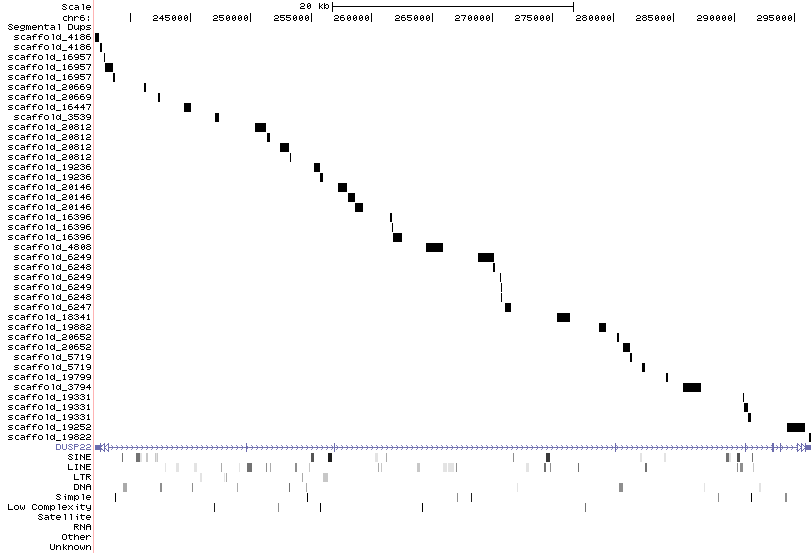
\includegraphics[scale=0.45]{shatter.png}
\end{center}
\caption{Sadece Illumina platformu kullanılarak yapılan bir tüm genom birleştirmesi~\cite{Li2010b} sonucunda ortaya çıkan referanstaki DUSP22 geninin onlarca parçaya ayrıldığı görülmüştür~\cite{Alkan2011c}}
\label{fig:shatter}
\end{figure}



Bunlara rağmen her YND teknolojisinin diğerlerine göre bazı avantajları vardır. Örneğin Illumina platformu en çok veriyi en ucuza üretebilir (10 günde 600 milyar baz çiftinden fazla) ve baz okuma hata oranı en azdır (\%0.1). 454 cihazı diğerlerine göre daha büyük molekülleri eşli dizileyebilir (yaklaşık 20.000 baz çifti). Pacific Biosciences ise şu anki teknolojiler arasında ürettiği ortalama dizi uzunluğu en fazla olan platformdur (1.4 kb) ve ``grup dizileme'' (strobe sequencing) teknolojisi ile eşli dizilemeye (paired-end sequencing) göre bir molekülden daha fazla bilgi çıkarabilir (Şekil~\ref{fig:strobe}). Bu nedenledir ki, aynı anda birden fazla teknoloji ile elde edilmiş verileri kullanmak, her bir teknolojinin diğerlerine üstün yanlarından faydalanıp, sahip olduğu dezavantajları da diğer teknolojilerin avantajları ile gidermek en uygunu olacaktır. Örneğin Illumina'nın sağladığı yüksek kalitedeki baz okuma doğruluğu ile Pacific Biosciences'ın \%15'lik hata oranını düzelterek, aynı zamanda Pacific Biosciences'in gruplu ve uzun dizileme özelliği sayesinde Illumina'nin kısa dizilerinin birleştirilmesini geliştirip tekrarlı alanlardaki yapısal birleştirme hatalarını en aza indirgemek mümkün olacaktır.

\begin{figure}[htb]
\begin{center}
  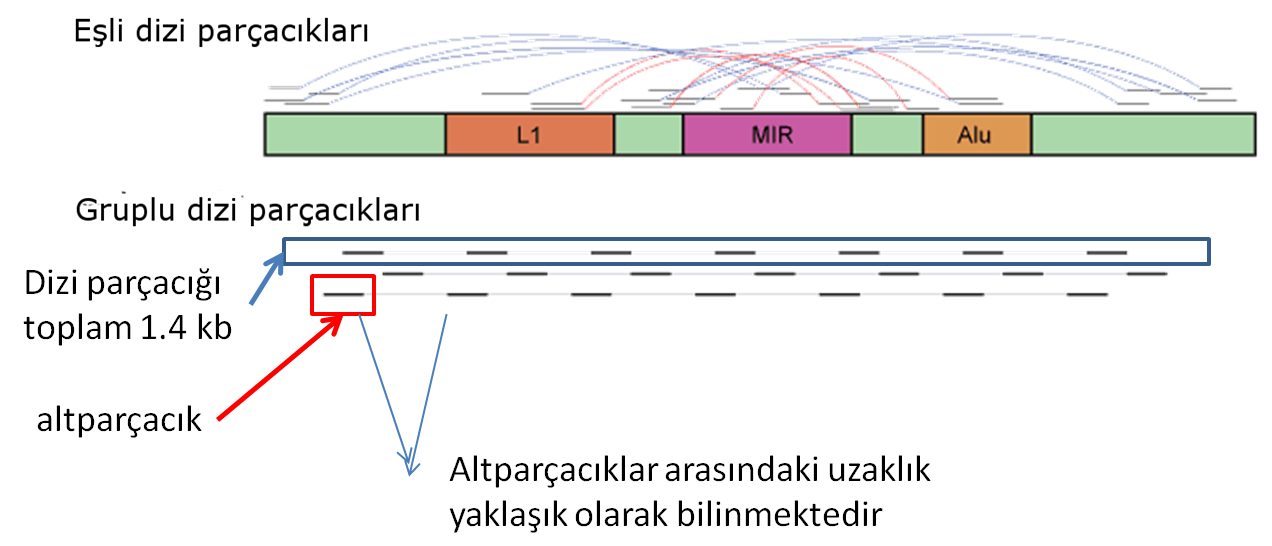
\includegraphics[scale=0.75]{strobe.png}
\end{center}
\caption{Eşli dizileme (paired-end sequencing) ve gruplu dizileme (strobe sequencing). Illumina, Ion Torrent, 454, Complete Genomics ve SOLiD cihazları ile eşli dizileme yapilabilinirken, Pacific Biosciences gruplu dizilemeyi desteklemektedir.}
\label{fig:strobe}
\end{figure}



\clearpage


\begin{center}
{\bf \Large 3. GEREÇ VE YÖNTEM} 
\end{center}
\addcontentsline{toc}{section}{3. GEREÇ VE YÖNTEM}
\noindent

\noindent
{\bf \large 3.1. Ekzom Dizilemede GC ve Yakalama Verimi Hatalarının Düzeltilmesi}
\addcontentsline{toc}{subsection}{3.1 Ekzom Dizilemede GC ve Yakalama Verimi Hatalarının Düzeltilmesi}

DNA'nın sadece belirli bölgelerinde yaşanan dizi değişimlerine bakmak için tüm genom birleştirme yöntemini kullanmak yerine hedefleyici birleştirme yöntemini kullanmak daha etkin sonuçlar vermektedir. Hedefleyici birleştirme yönteminin alt sınıflarından birisi de yalnızca protein kodlayan bölgeleri hedefleyen ekzom birleştirme yöntemidir. Ancak ekzom birleştirme metodunu kullanabilmek için ekzon verilerindeki GC-içeriği ve ekzon yakalama etkinliği gibi bazı sapmaları düzeltmek gerekmektedir (Şekil~\ref{fig:exomedepth}). Bu sapmalardan GC-içeriğini düzeltmek için yapılmış birçok çalışma olmasına rağmen~\cite{Krumm2012,Fromer2012} ekzon yakalama etkinliğiyle alakalı bilinen bir çalışma bulunmamaktadır. Bu alandaki açığı kapatarak ekzom birleştirme yöntemini de kullanabilmek için bir çalışma yaptık. Prob yakalama etkinliğinde varolan sapmaları düzeltmek için yaptığımız bu çalışma sonucunda bu etkiyi büyük ölçüde düzelttik. 


\begin{figure}[htb]
\begin{center}
  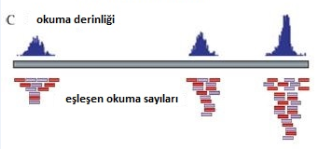
\includegraphics[scale=0.75]{exomedepth.png}
\end{center}
\caption{Okumaların 3 farklı ekzom bölgesine eşleştirilmesi. Her üç ekzonun da kopya sayısı aynı olmasına rağmen GC profili ve yakalama etkinliğindeki farklılıklar nedeniyle dizileme derinlikleri farklı görünebilmektedir.}
\label{fig:exomedepth}
\end{figure}

 Prob yakalama etkinliği, genomun her yerinde o bölgede kullanılan probun özelliklerine göre değişmektedir. Her bölgenin bu sapmadan ne kadar etkilendiğini görmek ve bu sapmaları düzeltebilmek için, dizileme teknolojileri kullanılarak elde edilen DNA parçacıklarını ekzon koordinatlarına göre eşleştirdik. Daha sonra her bir bölgeye ait prob sayısı ve dizi derinliğine bakılarak, yakalama etkinliklerini tespit ettik. 

{\bf 3.1.1. Birden Fazla Örnek Üzerinde Çalışabilmek için Ekzom Dizileme Verilerinin Uyarlanması}
\addcontentsline{toc}{subsubsection}{3.1.1. Birden Fazla Örnek Üzerinde Çalışabilmek için Ekzom Dizileme Verilerinin Uyarlanması}

Ekzom dizilemesi verilerinin üzerinde çalışırken, örneklere ait verilerin okuma derinlikleriyle kopya sayısı varyantlarını kıyaslayabilmek için pencere büyüklüklerini (window size) eşitlememiz gerekmektedir. Bunu yapabilmek için her bir ekzona map edilmiş olan okuma sayısının ortalaması (exome mean read count)(EMRC) hesaplanmalıdır. EMRC aşağıdaki gibi formülize edilmiştir:

\[ERMC_e = \frac{RC_e}{L_e}\]

Burada $RC_E$ hedeflenen e genomik bölgesine eşleştirilen okuma sayısını, $L_e$ ise aynı genomik bölgenin büyüklüğünü ifade etmektedir. EMRC genomun edeflenen her bir bölgesi için hesaplanıp, belirli bölgelere eşleştirilen okuma yoğunluğunun bir ölçüsünü vermektedir. 

{\bf 3.1.2. GC İçeriği Yanlılığı}
\addcontentsline{toc}{subsubsection}{3.1.2 GC İçeriği Yanlılığı}

GC içeriği yanlılığı, okuma kapsamı (read coverage) ile dizileme verisinde bulunan GC içeriğinin arasındaki ilişkiyi ifade etmektedir. Bu yanlılık, DNA dizilemesinde varolan kopya sayısı tahmininde de olabileceği gibi, genomdaki parça (fragment) bolluğunu ölçmeye odaklı analizlerdeki sinyalleri domine edebilmektedir. Ayrıca örnekler arasında tutarlılık gösteren bir yanlılık olmayıp, tek bir örnekteki yanlılığı ortadan kaldırabilecek en iyi yöntem diye bir şeyden de söz edilememektedir.

{\bf 3.1.3. Batch Etkisi}
\addcontentsline{toc}{subsubsection}{3.1.3 Batch Etkisi}

Genetik varyantlar, gen ve protein ifadelerinde ve epigenetik modifikasyonlar için geniş ölçekte kullanılan  YND teknolojileri, gözden kaçırılabilecek batch etkisine sık sık maruz kalabilmektedir. Batch yanlılığı laboratuvar şartlarından ve personel değişimleri gibi durumlardan meydana gelebilmektedir. Bu etki,  verdiği doğru olmayan sonuçlara bağlı olarak çok önemli bir problem haline gelmiştir.


{\bf 3.1.4. Temel İçerik Analizi (Principal Component Analysis)(PCA)}
\addcontentsline{toc}{subsubsection}{3.1.4 Temel İçerik Analizi (Principal Component Analysis)(PCA)}

Temel içerik analizi, modern veri analizinin dayanak  noktası haline gelmiştir. Bunun yanı sıra uygulamalı lineer cebirin en değerli sonucu olarak da kabul edilmektedir. PCA olarak da bilinen bu yöntem çok yaygın bir şekilde ancak çok iyi anlaşılmadan kullanılmaktadır. Bu da yanlış sonuçlar doğurmaktadır. Yürütmekte olduğumuz çalışmada PCA yönteminin olası yanlış kullanımlarını düzelterek, daha doğru veriler de elde etmeyi hedeflemekteyiz. Karmakarışık bir veri kümesinden, en alakalı kısmı alabilen parametrik olmayan bir metot olduğu için nöroloji biliminden bilgisayar grafiği alanına kadar geniş bir yelpazede kullanılmaktadır. Minimal düzeyde ek bir çaba ile PCA, kompleks bir veri kümesinden kümeyi ifade edebilen küçük bir data setini elde edebilmeyi, zaman zaman ise gizli kalmış altta yatan basit dinamiklerin ortaya çıkarılmasını sağlamaktadır. PCA'nın amacı,  pürüzlü (noisy) veri kümesini en anlamlı ve daha basit bir şekilde yeniden ifade edebilmeyi sağlamaktır.


{\bf 3.1.5. Değişken Bayes Çıkarımı}
\addcontentsline{toc}{subsubsection}{3.1.5. Değişken Bayes Çıkarımı}


Tekil değer ayrışımı (SVD), bir matrisin optimal bir şekilde düşük rank ayrımını (karesel hata anlamında), döndüren bir matris  ayrıştırma algoritmasıdır. SVD'nin; çıktısı, verinin kompakt ve bilgilendirici bir gösterimi olarak yorumlanabilecek makine öğrenimi uygulamalarında geniş bir kullanımı vardır. Maalesef bunun yanında, aşırı aralıklı matrisler için veriye gereğinden fazla uyumlu grafikler ortaya çıkararak, yeni verinin grafikte doğru bir şekilde yer bulmasını engelleyebilmektedir. Bu nedenle çok dikkatli bir şekilde ele alınmalıdır. Kopya sayısı varyantı tespiti algoritmalarında da  oldukça fazla kullanılmaktadır.

Elimizde var olan (kopya sayısı) $\times$ (örnekler) matrisinin  ekzom datasına bağlı olarak gelişen aralıklı yapısından dolayı SVD bazen yeterli olamamaktadır. Burada oluşabilecek verinin fazla uyumlu grafikler ortaya çıkarabilmesi durumunu engelleyebilmek için her biri veri kümesinin yapısına uygun parametreler ve yapılar ortaya çıkaran değişken bayes çıkarımını kullanmayı planlamaktayız. Elimizdeki veri kümesine oldukça benzeyen daha önce internet sitelerinde yer alan sinema tavsiyeleri için makine öğrenmesi uygulamasında da kullanılmış ve buradaki sonuçları iyileştirmiştir.

{\bf 3.1.6. GC ve yakalama etkinliğinden doğan farklılıkların düzeltilmesi}
\addcontentsline{toc}{subsubsection}{3.1.6. GC ve yakalama etkinliğinden doğan farklılıkların düzeltilmesi}

Elimizdeki veriyi matris benzeri bir yapı olarak düşünebiliriz. Bunlardan ilki; (okuma derinliği) $\times$ (örnek), ikincisi; (kopya sayısı varyantı) $\times$ (örnekler) matrisidir  diyebiliriz. Okuma derinliği verisini içeren ilk matrisimizde eksik veri bulunmamaktadır. Amacımız ilk matristeki verileri kullanarak, fazla sayıda eksik veri içeren ikinci matrisimizdeki kopya sayısı varyantlarını tespit edebilmektir. Elimizde varolan veriler tüm genom dizilemesi verileridir. Biz bu verileri daha önceden elde edilmiş insan ekzom verisiyle eşleştirdik(mapping). Böylece kopya sayısı varyantı tespitinde daha avantajlı DNA'nın sadece ekzom kısmıyla ilgilenebiliyoruz. Eşleştirdikten sonra matrislerin üzerinde işlem yapabilmemiz için farklı örneklerden  geliyor olmasından kaynaklanan pencere büyüklüğü sorununu çözebilmek için daha önce bahsetmiş olduğumuz ``Birden Fazla Örnek Üzerinde Çalışabilmek için Ekzom Dizileme Verilerinin Uyarlanması'' kısmındaki EMRC formülünü kullanarak uniform matrisler elde etmekteyiz.

Bilindiği üzere kromozomlar eşey ve otozomal kromozomlar olarak iki grupta toplanmaktadır. Bu iki tür kromozom farklı yapılarından dolayı ayrı ayrı ele alınmalıdır. Bu sebeple ilk aşamada otozomal kromozomlar üzerinde çalışacağımız için ekzon dizilemesinden eşey kromozomları olan X ve Y kromozomlarına dair veriler çıkarıldı. 

Elimizde bulunan kopya sayısı varyantı verilerinde 2, normal kopya sayısı; 0-1 delesyon; 3 ve daha fazlası duplikasyon görüldüğünü belirtmektedir. 1000 Genom Projesi'nden~\cite{1000GP2012} mevcut populasyonlara ait örneklemlerin (sample) deletion kısımları alındı. Daha sonra bu deletionların arasından bütün örneklemlerde ortak olarak görülen deletionlar alındı. Alınan bu deletionlar ile daha önceden elde etmiş olduğumuz verilerin kesişmeyen kısımları ``normal'' yani 2 olarak kabul edildi.

Bu veri kümesinde GC ve yakalama prob sayıları ile dizileme derinliği arasındaki ilişkiyi anlayabilmek için ykarıda anlatıldığı üzere kopya sayısı varyasyonu bulunmayan bölgelerde korelasyon hesaplaması yaptık. Bu bölgelerde varyasyon bulunmadığı için normal dağılımda tüm ekzonların dizileme derinliğinin aynı olması beklenir, ancak GC değerleri ve yakalama prob sayılarının farklılıkları nedeniyle farklı derinlikler gözlenmektedir (Şekil \ref{fig:exomedepth}). Korelasyon katsayılarını aşağıdaki şekilde hesapladık:

\[r_{rd,pr} = \frac{\sum_{i=1}^{n}(rd_i-\overline{rd})(pr_i-\overline{pr})}{\sqrt{\sum_{i=1}^{n}(rd_i-\overline{rd})^2\sum_{i=1}^{n}}(pr_i-\overline{pr})^2} \]
\[r_{rd,gc} = \frac{\sum_{i=1}^{n}(rd_i-\overline{rd})(gc_i-\overline{gc})}{\sqrt{\sum_{i=1}^{n}(rd_i-\overline{rd})^2\sum_{i=1}^{n}}(gc_i-\overline{gc})^2} \]

\paragraph{Çoklu korelasyon.}
Çoklu korelasyon bir bağımlı değişkenin çok sayıda bağımsız değişken ile arasındaki lineer bağlamı ölçer. Bu şekilde modelde birden fazla değişkenin kullanılıp kullanılmayacağına karar vermek için kullanılır. GC içerigi (gc) ve prob sayısını (pr) bağımsız, dizileme derinliğini (rd) bağımlı değişken olarak alıp çoklu korelasyon katsayısını aşağıdaki şekilde hesapladık:

\[R_{rd,pr,gc} = \frac{\sqrt{r_{rd,gc}^2 + r_{rd,pr}^2 - 2r_{rd,gc}r_{rd,pr}r_{gc_pr}}}{\sqrt{1-r_{gc,pr}^2}}\]

Burada $r_{rd,gc}$ derilik ve GC arasında, $r_{rd,pr}$ derinlik ve prob sayısı arasında, $r_{gc,pr}$ de GC ve prob sayısı arasındaki ikili korelasyonu ifade eder.

\paragraph{Veri düzleştirme (LOESS).} 
LOESS metodu yerel ağırlıklı lineer gerileme kullanarak verilerin düzleştirilmesini sağlar. Düzlük katsayısı dışında bir parametreye ihtiyaç duymaz. Verinin aşağıdaki gibi bir fonksiyon ile üretildiği varsayılır:

\[y_i = g(x_i) + \epsilon_i\]

Burada $g$, bağımsız değişkenler arasındaki düzlük katsayısını ifade eden bir fonksiyondur.

%LOESS metodu ile veri düzeltme işlemi aşağıdaki gibidir:

%$x_i$'nin $n$ farklı değişken ve $y_i$'in hesaplanan değer olduğu durumda:

%\begin{enumerate}
%\item
%  0 ve 1 arasında bir düzlük katsayısı seçilir (\alpha) Daha sonra $k$ değeri $\alpha\times n$ %değerine eşit ya da daha az olacan şekildeki en büyük tamsayı olarak hesaplanır.
%\item
%  Veri kümesindeki her $x_0$ için en yakın $k$ nokta bulunur. 
%\item
%\item
%\item
%\item
%\item
%\end{enumerate}

\begin{center}
{\bf \Large 4. BULGULAR}
\end{center}
\addcontentsline{toc}{section}{4. BULGULAR}
\noindent

\noindent
{\bf \large 4.1. }
\addcontentsline{toc}{subsection}{4.1 Ekzom Dizilemede GC ve Yakalama Verimi Hatalarının Düzeltilmesi}

\paragraph{Korelasyon değerleri} 

 Şekil \ref{fig:captureeff}'de 1000 Genom Projesi'ne~\cite{1000GP2012} ait rastgele seçilmiş 7 örneğe ait her bir ekzon bölgesindeki prob etkinliği ve dizi derinliği grafikte gösterilmektedir. Ayrıca korelasyon katsayıları da Tablo~\ref{tab:correlation}'da verilmiştir. Bu verilerdeki gürültüleri azaltabilmek için 1000 genom projesi kapsamındaki örneklerin her birinde ortak olarak bulunan delesyon, insersiyon ve düşük kapsama bölgeleri çıkarıldı. 

\begin{figure}[htb]
\begin{center}
  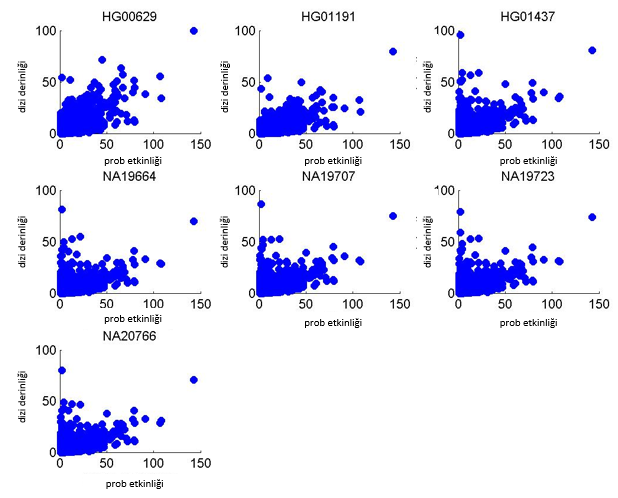
\includegraphics[scale=0.65]{captureeff.png}
\end{center}
\caption{Her bir ekzon bölgesine ait dizi derinliği ve prob yakalama etkinliği.}
\label{fig:captureeff}
\end{figure}

\begin{table}[htb]
\begin{center}
\begin{tabular}{|l|c|c|}
\hline 
{\bf Örnek } & {\bf RD-PR} & {\bf RD-PR-GC}\\
\hline 
HG00629 & 0.6478 & 0.7118\\
HG01191 & 0.6375 & 0.7095\\
HG01437 & 0.6483 & 0.6708\\
NA19664 & 0.6383 & 0.6640\\
NA19707 & 0.6484 & 0.6733\\
NA19723 & 0.6508 & 0.6751\\
NA20766 & 0.6509 & 0.6768\\
\hline
\end{tabular}
\end{center}
\caption{1000 Genom Projesi'nden 7 örneğin dizileme derinliği (RD), prob sayısı (PR) ve GC içeriği (GC) ile korelasyonları. Görüldüğü üzere PR ve GC değerleri birlikte alınıp çoklu korelasyon hesaplandığında daha yüksek korelasyon katsayısı elde edilmektedir.}
\label{tab:correlation}
\end{table}

 Şekil \ref{fig:captureeff}'de de görüldüğü gibi gürültünün azaltılmasına rağmen prob kapsama etkinliği ve dizi derinliği arasında yeteri kadar güçlü bir ilişki bulunamamıştır. Daha sonra genom üzerinde bulunan her bir bazın kendisine yakın olan dizilimlerden etkilendiği düşüncesinden yola 
çıkarak, her bir genin içindeki ekzonları bir bütün olarak düşündük (Şekil \ref{fig:captureeffgene}).

\begin{figure}[htb]
\begin{center}
  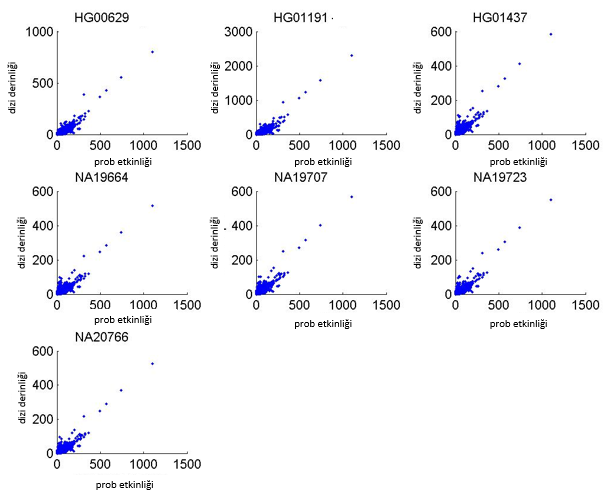
\includegraphics[scale=0.65]{captureeff-gene.png}
\end{center}
\caption{Her bir gen bölgesine ait dizi derinliği ve prob yakalama etkinliği.}
\label{fig:captureeffgene}
\end{figure}

  Sonuç olarak ekzonları ayrı ayrı ele almak yerine her bir gen bölgesinde bulunan ekzonları bir bütün olarak gördüğümüzde prob yakalama etkinliği ve dizi derinliği arasındaki ilişkinin güçlendiğini gözlemledik. Daha sonra datada bulunan prob etkinliği sapmasını düzeltebilmek için LOESS metodunu kullandık ve dizileme derinliğindeki hataları önemli ölçüde giderdik (Şekil~\ref{fig:captureeffloess}). Bu yöntem serpme diyagramında yerel olarak pürüzleri düzeltmede kullanılmaktadır.


\begin{figure}[htb]
\begin{center}
  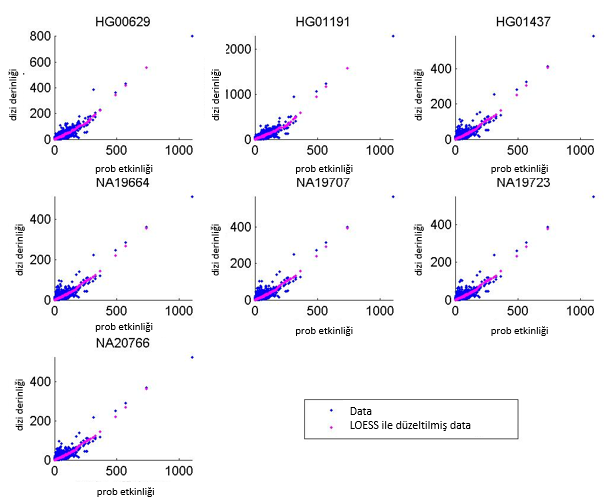
\includegraphics[scale=0.65]{captureeff-loess.png}
\end{center}
\caption{LOESS yöntemi kullanılarak düzeltilen veriler.}
\label{fig:captureeffgeneloess}
\end{figure}

LOESS metoduyla düzeltilen data kullanılarak, ekzom birleştirme yöntemini daha doğru bir şekilde yapmak mümkün olacaktır.

\begin{center}
{\bf \Large 5. TARTIŞMA/SONUÇ}
\end{center}
\addcontentsline{toc}{section}{5. TARTIŞMA/SONUÇ}

\noindent
Yürürlükte olduğu üç sene boyunca, **** projesinin ele aldığı soruların bir kısmında kayda değer bir ilerleme kaydetmiştir. 

\noindent
{\bf \Large 5.1. Öneriler}
\addcontentsline{toc}{section}{5.1. Öneriler}

{\small 
\bibliographystyle{plain}
\bibliography{calkan}

}




\label{endsectionb1}
\end{document}
